\lecture{13}{18/11/2021}
\vspace{0.5cm}
\noindent A questo punto promuoviamo le nostre variabili a operatori (con commutatore $[\hat n, \hat \delta]=-i$):
\begin{equation*}
    \hat p = - i \hbar \partialderivative{\delta} \qquad \hat n = - i \partialderivative{\delta} 
\end{equation*}
E in questo modo possiamo riscrivere l'hamiltoniana (sempre divisa in un termine cinetico e in un termine potenziale):
\begin{equation*}
    \hat H = E_C \hat n ^ 2 - E_J \left( \cos{\hat\delta} + \frac{I_B}{I_0}\hat\delta \right)
\end{equation*}
Con questa forma è molto più semplice capire cosa succede all'energia potenziale con l'applicazione di una corrente di bias: inizialmente essa ha un profilo prettamente sinusoidale (con molti livelli metastabili ed equidistanti); con la corrente, invece, si deforma asimmetricamente come in Figura \ref{fig:phase_qubit_pot}.
\begin{figure}[H]
    \centering
    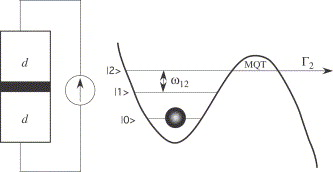
\includegraphics[width=0.5\textwidth]{images/phase_qubit_pot.jpg}
    \caption{}
    \label{fig:phase_qubit_pot}
\end{figure}
\noindent Ricordando l'effetto Josephson per cui $V = \frac{\hbar \dot \delta}{2e}$, avremo che una coppia di Cooper si romperà nel caso in cui $eV > \Delta$ (con $\Delta$ che rappresenta il gap fra le due buche) per un effetto che chiameremo MQT (\textit{Macroscopic Quantum Tunneling}).
Modificando la corrente di bias nel modo adeguato potremo facilmente regolare l'hamiltoniana in modo da avere soltanto pochi livelli metastabili (ciò si ottiene sperimentalmente con $I_b \sim 0.95 I_0$).
Derivando in $\delta$ l'hamiltoniana è facile verificare che il minimo si troverà in corrispondenza di $\delta_{min} = \arctan{\frac{I_B}{I_0}}$. \\
Definendo ora una nuova variabile $\eta = \delta - \delta_{min}$ possiamo scrivere il potenziale come (espandendo in $\eta$):

\begin{equation*}
    U(\eta) \sim -E_J \left( \sqrt{1 - \left( \frac{I_b}{I_0}\right)^2}\frac{\eta^2}{2}+ \frac{I_b}{I_0} \frac{\eta^3}{6}+\cdots \right)
\end{equation*}
Potenziale compatibile con un oscillatore armonico con $\omega_0 = 1/\sqrt{L_{J0}C}$ se non c'è corrente di bias, a cui è aggiunta un'anarmonicità del terzo ordine con la corrente. Con la corrente di bias abbiamo ($L_{J0}= \frac{\hbar}{2eI_0}$):
\begin{equation*}
    \omega_I^2 = \omega_0 ^ 2 \sqrt{1 - \left( \frac{I_b}{I_0}\right) ^ 2} = \omega_0 ^2 \cos \delta = \frac{1}{L_J C} < \frac{1}{L_{J0}C}
\end{equation*}
L'anarmonicità data dalla corrente di bias porta a una differenza fra le prime due frequenze di transizione nell'ordine dei $300\text{ MHz}$ (sono dunque facilmente distinguibili).
Un'altra relazione che si può ottenere è relativa alla probabilità di decadere da uno degli stati metastabili: $\Gamma_{n+1} \sim 1000 \Gamma_n$. Ovvero ogni stato eccitato decade con una probabilità mille volte superiore rispetto al livello energetico immediatamente inferiore.
Avendo un qubit costruito in questo modo, siamo in grado di misurare con relativa facilità la distribuzione delle coppie di Cooper fra i primi due livelli. Ci basta irradiare il circuito alla frequenza di transizione $\omega_{12}$: se lo stato che descrive il sistema è $\ket 0$ non vedremo alcuna accelerazione del rate di decadimento, se invece siamo in $\ket 1$ ecciteremo il sistema a $\ket 2$ con una differenza di \textit{decay rate} misurabile. \\
Ugualmente possiamo irradiare a frequenza costante cambiando la corrente di bias.
In una misura, il circuito va leggermente modificato in modo da disaccoppiare il circuito superconduttivo con la strumentazione di misura. In ogni caso, comunque, nel circuito finale non è presente alcuna "isola" (conduttore isolato): le coppie di Cooper possono, perciò, variare senza problemi in numero.
Diamo un attimo qualche numero sulla capacità da usare. La condizione che vogliamo ottenere è che $E_0$ (energia del primo livello metastabile) sia molto minore di $E_J$ (l'energia della barriera di potenziale fra "i due minimi"). $E_0 \ll E_J$ è equivalente a dire: $\frac{\hbar \omega_0}{2}= \sqrt{8 E_C E_J} \ll E_J$, ma siccome $E_C \propto \frac{1}{C}$ non possiamo diminuire la capacità eccessivamente. Tipicamente si usano capacità $\sim 10\text{ pF}$ (piuttosto grandi rispetto alla media).

\subsection{Charge qubit: Cooper Pair Box}

Il secondo tipo di circuito che analizzeremo sarà la cosiddetta  \textit{Cooper Pair Box}.
Il circuito è ottenuto con due elettrodi separati da un dielettrico (il che porta a una capacità chiamata \textbf{gate capacity} $C_g$). Il fatto che siano superconduttori non è ora strettamente necessario.
Sul primo elettrodo è collegato un generatore di tensione. Sul secondo elettrodo viene depositato (isolato in modo da creare una giunzione Josephson) un altro superconduttore collegato anch'esso al generatore.

\begin{figure}[!ht]
    \centering
    \subfloat[\centering]{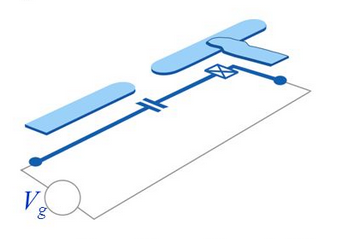
\includegraphics[width=0.5\textwidth]{images/cooper_pair_box.png}}%
    \qquad
    \subfloat[\centering]{
        \begin{circuitikz}
        \draw (0,0)
        to[barrier] (0,2) % The L source
        to[short] (2,2)
        to[C=$C_J$] (2,0) % The resistor
        to[short] (0,0)
        node[ground]{} (-1.5, 0) node[ground]{}
        to[V=$V_g$] 
        (-1.5,2.5)  
        to[C=$C_g$] (0.5,2.5) -- (0.5,2);
        \end{circuitikz}
    }
\end{figure}
\noindent Il termine cinetico dell'hamiltoniana del circuito è leggermente diverso e porta a:
\begin{equation*}
K =\frac{CV^2}{2}+ C_g \frac{(V_g - V)^2}{2} = \frac{C_{tot}}{2} \left( \frac{\hbar }{2e}\dot \delta - \frac{C_g}{C_{tot}}V_g \right) ^2 
\end{equation*}
dove $n_g = \frac{C_g}{2e}V_g$  rappresenta il numero di coppie di Cooper nella capacità di gate.
Perciò possiamo scrivere tutto come prima, ma identificando il momento come:
\begin{equation*}
    \hat p = \hbar(\hat n-n_g)
\end{equation*}
e dunque
\begin{equation*}
    \hat K = E_C(\hat n-n_g)^2
\end{equation*}
L'hamiltoniana risulta quindi
\begin{equation*}
    \hat H = E_C ( \hat n - n_g)^2 - E_J \cos \hat \delta
\end{equation*}
Notiamo un particolare andamento dell'energia: se rimuoviamo la giunzione Josephson ($E_J=0$) otteniamo un'energia "a parabola" per ciascun valore fissato di $\hat n$ (facendo variare $n_g$ col potenziale esterno). Le parabole si intersecano tutte e, se reintroduciamo la giunzione Josephson, potremo saltare da una all'altra nei punti in cui l'energia è degenere: fondamentalmente attraverso la giunzione potranno saltare dentro e fuori dall'isola le coppie di Cooper. Per ogni parabola avremo infiniti punti di degenerazione (con le parabole immediatamente adiacenti e con quelle più lontane).
Tali punti corrispondono ai valori per cui il sistema assume uno stato in sovrapposizione con diversi $\hat n$. Aggiungendo il \textit{tunneling} apriamo dei gap (che crescono con $\frac{E_J}{E_C}$) interni alle parabole e otteniamo un andamento dell'energia descritto in Figura \ref{fig:spectrum_CPB}\footnote{Osserviamo la grande similarità con i risultati dello schema degli elettroni quasi liberi in Fisica dello Stato Solido.}.
\begin{figure}[H]
    \centering
    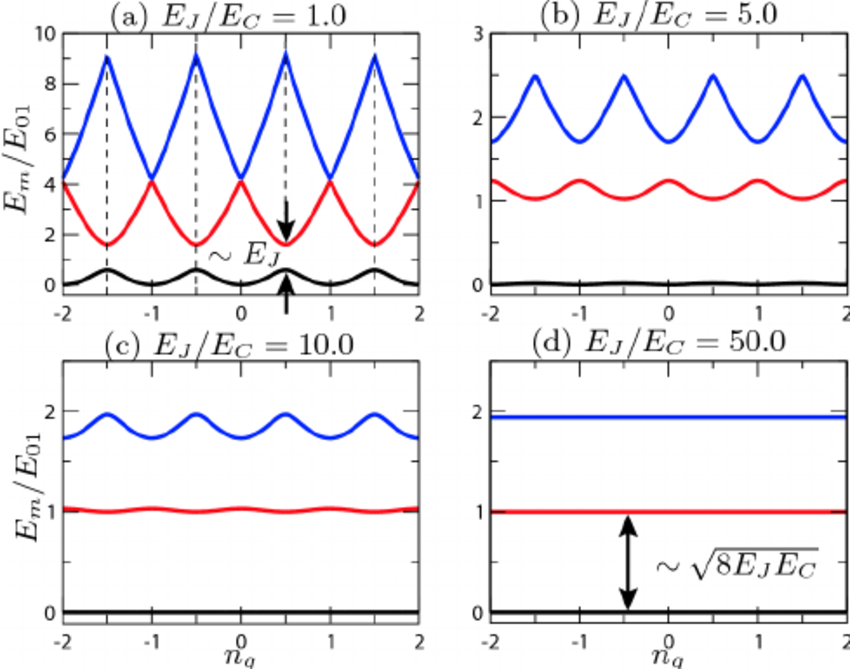
\includegraphics[width=0.7\textwidth]{images/Energy-spectrum-CPB.png}
    \caption{Convoluzione degli spettri energetici per una CPB.}
    \label{fig:spectrum_CPB}
\end{figure}
\noindent Dunque, se aumentiamo la capacità da cui dipende $E_C$ il sistema perde sempre più dipendenza dalla carica (ottimo, stiamo riducendo uno dei principali elementi di \textit{dephasing}), ma anche l'anarmonicità diminuisce. Il limite $E_J / E_C \rightarrow \infty$ viene detto \textit{transmon limit} ed è quello attualmente utilizzato nei qubit superconduttivi.